\documentclass[letterpaper, 12pt]{math}

\usepackage{tikz}

\title{Multivariable and Vector Calculus}
\author{Alvin Lin}
\date{August 2017 - December 2017}

\begin{document}

\maketitle

\section*{Functions of Several Variables}
A function of a single variable:
\begin{center}
  \begin{tikzpicture}
    \draw (0,0) -- node[below] {x} (2,0) -- node[right] {x} (2,2) --
      (0,2) -- (0,0);
  \end{tikzpicture}
\end{center}
\[ A(x) = x^2 \]
A function of two variables:
\begin{center}
  \begin{tikzpicture}
    \draw (0,0) -- node[below] {x} (4,0) -- node[right] {y} (4,2) --
      (0,2) -- (0,0);
  \end{tikzpicture}
\end{center}
\[ A(x,y) = xy \]
Even for functions of many variables, they still have properties such as domain
and range.
\[ f(x,y) = \frac{1}{\sqrt{1-x^2-y^2}} \]
Domain:
\[ 1-x^2-y^2 > 0 \therefore x^2+y^2 < 1 \]
Range:
\[ [1,\infty) \]

\subsubsection*{Example}
Find the domain of the function:
\[ f(x,y) = \frac{\ln(2-x)}{\sqrt{x-3y}} \]
\begin{align*}
  2-x &> 0 \\
  &\equiv x < 2\\
  x-3y &> 0 \\
  &\equiv y < \frac{x}{3}
\end{align*}
\begin{center}
  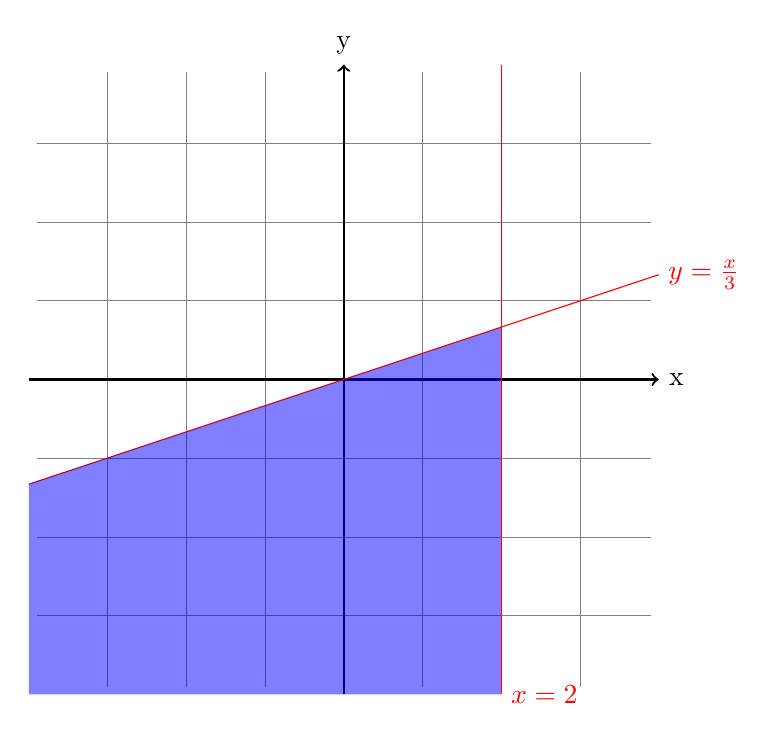
\begin{tikzpicture}
    \draw[step=1cm,gray,very thin] (-3.9,-3.9) grid (3.9,3.9);
    \draw[thick,->] (-4,0) -- (4,0) node[right] {x};
    \draw[thick,->] (0,-4) -- (0,4) node[above] {y};
    \draw[red] (2,4) -- (2,-4) node[right] {\( x = 2 \)};
    \draw[red] (-4,-1.33) -- (4,1.33) node[right] {\( y = \frac{x}{3} \)};
    \fill[opacity=0.5,blue] (-4,-1.33) -- (2,0.66) -- (2,-4) -- (-4,-4) --
      cycle;
  \end{tikzpicture}
\end{center}

\section*{Limits}

\subsubsection*{Example}
\[ \lim_{(x,y)\to(2,1)}\frac{xy}{x^2+2y^2} = \frac{1}{3} \]

\subsubsection*{Example}
\begin{align*}
  \lim_{(x,y)\to(0,0)}\frac{x^2+y^2}{\sqrt{1-x^2+y^2}-1} &=
    \lim_{(x,y)\to(0,0)}\frac{(x^2+y^2)(\sqrt{1-x^2-y^2+1})}
    {(\sqrt{1-x^2-y^2}-1)(\sqrt{1-x^2-y^2}+1)} \\
  &= \lim_{(x,y)\to(0,0)}\frac{(x^2+y^2)(\sqrt{1-x^2-y^2+1})}
    {1-x^2-y^2+1} \\
  &= -2
\end{align*}

\subsection*{Definition}
\[ lim_{(x,y)\to(x_{\circ},y_{\circ})} = L \]
is defined as for every \( \epsilon > 0 \) there exists \( \delta > 0 \) such
that \( |f(x,y)-L| < \epsilon \) if \( dist((x,y),(x_{\circ},y_{\circ}))
< \delta \). Notice that if:
\[ \lim_{(x,y)\to(x_{\circ},y_{\circ})}f(x,y) = L \quad\text{ and }\quad
  \lim_{(x,y)\to(x_{\circ},y_{\circ})}g(x,) = M \]
Then:
\[ \lim_{(x,y)\to(x_{\circ},y_{\circ})}\frac{f(x,y)}{g(x,y)} = \frac{L}{M} \]

\subsection*{Theorem}
If:
\[ \lim_{(x,y)\to(x_{\circ},y_{\circ})}f(x,y)\text{ on }C_1 \ne
  \lim_{(x,y)\to(x_{\circ},y_{\circ})}f(x,y)\text{ on }C_1 \]
Then \( \lim_{(x,y)\to(x_{\circ},y_{\circ})}f(x,y)\text{ on }C_1 \) does not
exist.

\subsubsection*{Example}
\[ \lim_{(x,y)\to(0,0)}\frac{xy}{x^2+2y^2} = \lim_{(x,y)\to(0,0)}\frac{0}{x^2} =
  \lim_{(x,y)\to(0,0)}\frac{0}{2y^2} = 0 \]
Inconclusive according to the theorem above. Take \( y = kx \):
\[ \lim_{(x,y)\to(x_{\circ},y_{\circ})}\frac{xkx}{x^2+2kx^2} =
  \lim_{(x,y)\to(x_{\circ},y_{\circ})}\frac{k}{1+2k} = \frac{k}{1+2k} \]
The original limit does not exist.

\subsubsection*{Example}
\[ \lim_{(x,y)\to(0,0)}\frac{x^2y}{x^2+2y^2} \]
Take \( y = kx \):
\[ \lim_{x\to0}\frac{x^2kx}{x^2+2k^2x^2} = \lim_{x\to0}\frac{kx}{1+2k^2} = 0 \]
Take \( y = kx^2 \):
\[ \lim_{x\to0}\frac{x^2kx^2}{x^2+2k^2x^4} = \lim_{x\to0}\frac{kx^2}{1+2k^2x^2}
  = 0 \]
By the Squeeze Theorem:
\[ \lim_{(x,y)\to(0,0)}0 \le \lim_{(x,y)\to(0,0)}\frac{x^2y}{x^2+2y^2} \le
  \lim_{(x,y)\to(0,0)}y \]
We can conclude that \( \lim_{(x,y)\to(0,0)}\frac{x^2y}{x^2+2y^2} = 0 \).

\section*{Partial Derivatives}
\[ \lim_{h\to0}\frac{f(x+h,h_{\circ})-f(x,y_{\circ})}{h} =
  \pdiff{f}{x}(x,y_{\circ}) \]
Examples:
\begin{align*}
  \pdiff{}{y}(x^2y^3-x^2+xy) &= x^23y^2+x \\
  \pdiff{}{x}(x^2y^3-x^2+xy) &= y^32x-2x+y \\
  \pdiff{}{x}(x^y) &= yx^{y-1} \\
  \pdiff{}{y}(x^y) &= x^y\ln(x)
\end{align*}
Extensions:
\[ \pdiff{}{x}\pdiff{f}{x} = \frac{\partial^2{f}}{\partial{x^2}} \]
\[ \pdiff{}{y}\pdiff{f}{y} = \frac{\partial^2{f}}{\partial{y^2}} \]
\[ \pdiff{}{y}\pdiff{f}{x} = \frac{\partial^2{f}}{\partial{y}\partial{x}} \]
\[ \pdiff{}{x}\pdiff{f}{y} = \frac{\partial^2{f}}{\partial{x}\partial{y}} \]

\subsection*{Clairaut's Theorem}
If \( \frac{\partial^2{f}}{\partial{x}\partial{y}} \) and \(
\frac{\partial^2{f}}{\partial{y}\partial{x}} \) are continuous in some
neighborhood of \( (x_{\circ},y_{\circ}) \), then:
\[ \frac{\partial^2}{\partial{x}\partial{y}}(x_{\circ},y_{\circ}) =
  \frac{\partial^2}{\partial{y}\partial{x}}(x_{\circ},y_{\circ}) \]
\( z = f(x,y) \) is called differentiable at \( x_{\circ},y_{\circ} \) if and
only if \( \pdiff{f}{x},\pdiff{f}{y} \) exist and are continouous at \(
(x_{\circ},y_{\circ}) \).

\subsubsection*{Example}
Check that \( u(x,t) = \sin(x-at) \) is a solution of:
\[ \frac{\partial^2{u}}{\partial{t^2}} =
  a^2\frac{\partial^2{u}}{\partial{x^2}} \]
\begin{align*}
  \frac{\partial^2{u}}{\partial{t^2}}(\sin(x-at)) &=
    \pdiff{u}{t}\cos(x-at)(-a) \\
  &= -\sin(x-at)(-a)(-a) \\
  &= -a^2\sin(x-at) \\
  a^2\frac{\partial^2{u}}{\partial{x^2}}(\sin(x-at)) &=
    a^2\pdiff{u}{x}\cos(x-at) \\
  &= a^2(-\sin(x-at)) \\
  &= -a^2\sin(x-at)
\end{align*}
Both derivatives are equal.

\subsubsection*{Example}
The temperature of a region is determined by:
\[ T(t) = \frac{60}{1+x^2+y^2} \]
A bug is located at (2,1), in which direction should it go to cool off.
\begin{align*}
  \pdiff{T}{x} &= \frac{-20}{3} \\
  \pdiff{T}{y} &= \frac{-10}{3}
\end{align*}
The bug should move towards the north and east.

\subsubsection*{Example}
\[ z = f(x,y) \quad x = x(t) \quad y = y(t) \]
The function \( z \) can be defined in terms of \( t \): \( z(t) \)
\begin{align*}
  \ddiff{z}{t} &= \lim_{h\to0}\frac{z(t+h)-z(t)}{h} \\
  &= \lim_{h\to0}\frac{f(x(t+h),y(t+h))-f(x(t),y(t))}{h} \\
  &= \lim_{h\to0}\frac{(f(x(t+h),y(t+h))-f(x(t+h),y(t)))(y(t+h)-y(t))}
    {h(y(t+h)-y(t))} \\
  &+\frac{(f(x(t+h),y(t))-f(x(t),y(t)))(x(t+h)-x(t))}{h(x(t+h)-x(t))} \\
  & \lim_{h\to0}\frac{(x(t+h)-x(t))}{h} = \ddiff{x}{t} \\
  & \lim_{h\to0}\frac{(y(t+h)-y(t))}{h} = \ddiff{y}{t} \\
  & \lim_{h\to0}\frac{(f(x(t+h),y(t))-f(x(t),y(t)))}{(x(t+h)-x(t))} =
    \pdiff{f}{x} \\
  \ddiff{z}{t} &= \pdiff{z}{x}\ddiff{x}{t}+\pdiff{f}{y}\ddiff{y}{t}
\end{align*}

\subsubsection*{Example}
\[ W = W(T,R) \quad \pdiff{W}{T} = -2 \quad \pdiff{W}{R} = 4 \]
\[ \ddiff{T}{t} = 0.1 \quad \ddiff{R}{t} = 0.5 \]
\[ \ddiff{W}{t} = \pdiff{W}{T}\ddiff{T}{t}+\pdiff{W}{R}\ddiff{R}{t} = 1.8 \]

\subsubsection*{Example}
Suppose you have a simple electric circuit:
\[ V = IR \quad R = 4.00\Omega \quad I = 0.08A \quad
  \ddiff{R}{t} = 0.03\frac{\Omega}{s} \quad \ddiff{V}{t} = -0.01V \]
What is \( \ddiff{I}{t} \)?
\begin{align*}
  I(V,R) &= \ddiff{I}{t} \\
  &= \pdiff{I}{V}\ddiff{V}{t}+\pdiff{I}{R}\ddiff{R}{t} \\
  &= \frac{1}{R}(-0.01)+\frac{-V}{R^2}{0.03} \\
  &= \frac{1}{400}(-0.01)-\frac{0.08}{400}(0.03)
\end{align*}

\subsubsection*{Example}
Suppose you have the surface
\[ x^3y^2z^4+4xy+z^2-6 = 0 \]
What is \( \ddiff{z}{y} \)?
\begin{align*}
  F(x,y,z(x,y)) &= 0 \\
  \ddiff{z}{y}F(x,y,z(x,y)) &=
    \pdiff{F}{x}\ddiff{x}{y}+\pdiff{F}{y}\ddiff{y}{y}+
    \pdiff{F}{z}\ddiff{z}{y} = 0 \\
  \ddiff{x}{y} &= 0 \\
  \ddiff{y}{y} &= 1\\
  \therefore \ddiff{z}{y} &= \frac{-\pdiff{F}{y}}{\pdiff{F}{z}} \\
  &= -\frac{F_y}{F_z} \\
  &= -\frac{x^3z^4(2y)+4x}{x^3y^2(4z^3)+2z}
\end{align*}

\subsubsection*{Example}
\[ y^2x^4+y^3x-2 = 0 \]
Find \( \ddiff{y}{x} \):
\begin{align*}
  2y\diff{y}{x}x^4+y^{2}4x^3+3y^2\ddiff{y}{x}x+y^3 &= 0 \\
  \ddiff{y}{x} &= \frac{-y^{2}4x^3-y^3}{2y+3y^{2}x}
\end{align*}

\subsubsection*{Example}
\[ S: F(x,y,z) = 0 \quad (x_{\circ},y_{\circ},z_{\circ})\in S \]
\[ C: \vec{r(t)} = \langle x(t),y(t),z(t)\rangle \quad C\subset S \quad
  (x_{\circ},y_{\circ},z_{\circ})\in S \]
\begin{align*}
  \pdiff{F}{x}\diff{x}{t}+\pdiff{F}{t}\pdiff{y}{t}+\pdiff{F}{z}\ddiff{z}{t} &=
    0 \\
  &= \langle\pdiff{F}{x},\pdiff{F}{y},\pdiff{F}{z}\rangle\cdot
    \langle\ddiff{x}{t},\ddiff{y}{t},\ddiff{z}{t}\rangle \\
  &= \gradientd{F}\cdot\overrightarrow{r'(t)} = 0 \\
  &\therefore \gradientd{F}\bot\overrightarrow{r'(t)}
\end{align*}

\subsubsection*{Example}
Check that every line normal to a sphere passes through its center.
\[ x^2+y^2+z^2-1 = 0 \]
\begin{align*}
  \vec{u} &= \gradientd{F} \\
  &= \langle2x,2y,2z\rangle \\
  l_{normal} &= \begin{cases}
    x &= x_{\circ}+t2x_{\circ} \\
    y &= y_{\circ}+t2y_{\circ} \\
    z &= z_{\circ}+t2z_{\circ}
  \end{cases} \\
  t &= -\frac{1}{2}
\end{align*}

\subsection*{Directional Derivative}
As an extension of the gradient definition:
\[ D_{\vec{u}}f = \gradientd{f}\cdot\vec{u} = |\gradientd{f}||\vec{u}|\cos\theta
  \quad |\vec{u}| = 1 \]
The maximum value of \( D_{\vec{u}} \) is \( |\gradientd{f}| \), which occurs
when:
\[ \vec{u} = \frac{\gradientd{F}}{|\gradientd{f}|} \]
The minimum value of \( D_{\vec{u}} \) is \( -|\gradientd{f}| \), which occurs
when:
\[ \vec{u} = -\frac{\gradientd{F}}{|\gradientd{f}|} \]

\subsubsection*{Example}
\[ z = x^2+y^2 \]
Find the directional derivative of \( z \) at (1,2) in the direction towards
(5,5).
\begin{align*}
  \vec{u} &= \langle5-1,5-2\rangle \\
  &= \langle\frac{4}{5},\frac{3}{5}\rangle \\
  D_z(1,2) &= \gradientd{z}\cdot\vec{u} \\
  &= \langle2x,2y\rangle\cdot\vec{u} \\
  &= \langle2,4\rangle\cdot\langle\frac{4}{5},\frac{3}{5}\rangle \\
  &= 4
\end{align*}

\begin{center}
  You can find all my notes at \url{http://omgimanerd.tech/notes}. If you have
  any questions, comments, or concerns, please contact me at
  alvin@omgimanerd.tech
\end{center}

\end{document}
